\documentclass[12pt]{article}

\usepackage{sbc-template}
\usepackage{amssymb}
\usepackage{graphicx,url}
\usepackage[spanish]{babel}
\usepackage[utf8]{inputenc}
% UTF-8 encoding is recommended by ShareLaTex
\usepackage{verbatim}
\usepackage{listings}
\usepackage{xcolor}

\definecolor{verde}{rgb}{0,0.5,0}

%para customizar o código (ver https://en.wikibooks.org/wiki/LaTeX/Source_Code_Listings)
\lstset{language=C, %defina a linguagem usada no trabalho
              belowcaptionskip=1\baselineskip,
                breaklines=true,
                frame=false,
                xleftmargin=\parindent,
                showstringspaces=false,
                basicstyle=\footnotesize\ttfamily,
                keywordstyle=\bfseries\color{green!40!black},
                commentstyle=\itshape\color{purple!40!black},
                identifierstyle=\color{blue},
                stringstyle=\color{orange},
                numbers=left,
            }

\sloppy

\title{Práctica 1 - Lógica Computacional}

\author{Arteaga Hernández Alejandro 313033414}

\begin{document} 

\maketitle
 \textbf{Ejercicio 1 \\}
\textit{Demuestra la correctud de la funcióńon mapeo definida en Haskell, es decir:\\
Para cualesquiera tipos a y b, funcíon f que dado un elemento de tipo a devuelve un
elemento de tipo b y lista l de tipo a, se cumple lo siguiente: \\
Si l = [x1, x2,..., xn] con xi elemento de tipo a,\\ entonces
mapeo  f l = [f x1, f x2, ..., f xn]\\}\\ 
Sea f una función tal que \\
f :: $A -> B$\\\\
suponemos que f() es correcta y también supondremos que la concatenación de listas es correcta\\\\
P.D que mapeo() es correcta\\
Caso Base :  Sea a tal que $a \in A $ y f(a) esta definida\\  mapeo([a]) = f(a) : [ ]\\ y como f(a) es correcta y la concatenación es correcta,
entonces mapeo([a]) es correcta.\\\\
Hipótesis de inducción: Suponemos que $mapeo([a_{0},a_{1}...a_{n}])$ es correcta\\
tal que $a_{i} \in A $ y que f($a_{i}$) está definida para todo $0\leq i \geq n$ 
\\
P.D que $mapeo([a_{0},a_{1}...a_{n},a_{n+1}])$ es correcta\\
$mapeo([a_{0},a_{1}...a_{n},a_{n+1}]) = [f(a_{0}),f(a_{1})...f(a_{n}),f(a_{n+1})))$\\
$mapeo([a_{0},a_{1}...a_{n},a_{n+1}]) = [f(a_{0}),f(a_{1})...f(a_{n})] : f(a_{n+1})$\\
$mapeo([a_{0},a_{1}...a_{n},a_{n+1}]) = mapeo([a_{0},a_{1}...a_{n}]) : f(a_{n+1})$\\
Pero $mapeo([a_{0},a_{1}...a_{n}])$ es correcta por la hipótesis de inducción, y como supusimos que f() era correcta y que la función concatenar también es correcta, entonces $mapeo([a_{0},a_{1}...a_{n}]) : f(a_{n+1})$ es correcta y por lo tanto
$mapeo([a_{0},a_{1}...a_{n},a_{n+1}])$ también es correcta $\blacksquare$
 \\\\\\\\\\\\\\\\\\\\\\\\
\\\\
 \textbf{Ejercicio 2 \\}
 \textit{Demuestra que la función alf es parcial y no inyectiva.\\}\\
 Sabemos que por definición, toda función es parcial.    Una función total sigue siendo parcial, pero no viceversa. 
 \\Podemos tomar el caracter 'a', que pertenece al conjunto que usa alf como dominio y veremos que alf('a') es indefinida
 en ese elemento del dominio, por lo tanto alf no es una función total pero sí una función parcial.
 \\La función alf() SÍ es inyectiva, supongamos que alf NO es inyectiva, como el dominio es finíto, podemos analizar todos los casos y demostrar que no existen 2 elementos del dominio a los cuales alf les asigne el mismo elemento en el codominio \\\\Para evaluar caso por caso, usaremos una función llamada map (En la parte de arriba ya he demostrado que es correcta), que recibe una función B y una lista A, y devuelve una lista con la evaluación de la función B con cada elemento de la lista A\\
 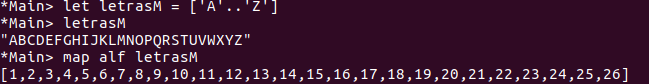
\includegraphics[width=16cm, height=2cm]{scren.png}\\
 \\Es evidente que todos los elementos de la lista otorgada por la función map() sobre la función alf() y la lista letrasM, son diferentes, y como para todo caracter que no esté contenido en esta lista, la función alf() no está definida, La función alf() es inyectiva\\\\
 \textbf{        Ejercicio 3\\}
 \textit{Demuestra que los operadores de suma y sucesor de números binarios, definidos
 en tu práctica, cumplen la siguiente propiedad:\\
 Dado x elemento de tipo BinPos se cumple que:\\
sucesor x = suma U x = suma x U}\\\\
Sucede porque yo lo definí así en la función xdxdxdxd\\
 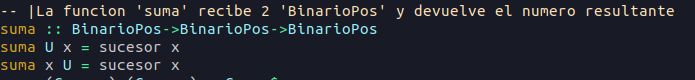
\includegraphics[width=16cm, height=2cm]{scren2.png}\\

 

\end{document}
